%-------------------------------------------------------------------------%
% ARCHIVO: img_tex/diagrama_completo.tex
% Versión corregida de ALTA FIDELIDAD - Método Hercule Poirot
%-------------------------------------------------------------------------%
\shorthandoff{>} % Evita conflictos con babel spanish

% 1. DEFINICIÓN DE DATOS GLOBALES
\newcommand{\puntosRegresion}{
    0.4/2.6, 0.4/3.0, 0.5/2.9, 0.5/2.4, 0.6/2.7, 0.7/2.5, 0.7/2.2, 0.8/2.7, 
    0.9/2.4, 1.0/2.2, 1.1/2.0, 1.2/1.5, 1.3/2.3, 1.3/1.9, 1.4/1.6, 1.5/2.1, 
    1.6/1.8, 1.7/1.5, 1.8/1.7, 1.8/2.2, 1.9/1.9, 2.0/1.5, 2.1/1.6, 2.2/2.1, 
    2.3/1.8, 2.3/2.5, 2.4/2.4, 2.4/2.7, 2.5/2.6, 2.5/2.9, 2.6/2.0, 2.7/1.8, 
    2.7/2.2, 2.8/2.4, 2.8/1.6, 2.9/1.3, 2.9/2.4, 3.0/1.4, 3.0/2.1, 3.1/1.6, 
    3.2/1.5, 3.3/1.1, 3.3/2.3, 3.4/1.3, 3.4/1.8, 3.5/0.8, 3.6/0.9, 3.6/1.2, 
    3.7/1.1, 3.8/0.6, 3.9/0.4, 4.0/0.5
}

% Trayectoria de la línea de predicción central
\newcommand{\lineaPrediccion}{
    (0.5, 2.8) .. controls (1.0, 2.0) and (1.5, 1.7) .. (2.3, 1.7)
               .. controls (3.0, 1.7) and (3.5, 1.2) .. (4.0, 0.7)
}

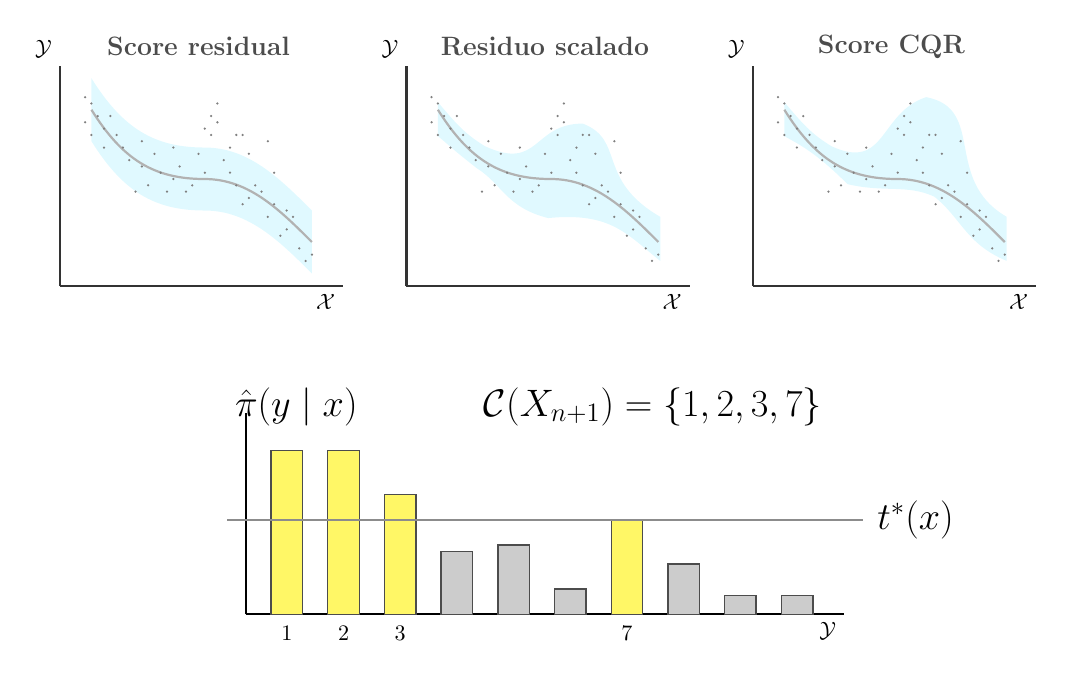
\begin{tikzpicture}[
    scale=0.8, every node/.style={transform shape},
    eje/.style={thick, draw=black!80},
    punto/.style={circle, fill=black!50, inner sep=0.4pt},
    barra_in/.style={draw=black!70, fill=yellow!60, line width=0.5pt},
    barra_out/.style={draw=black!70, fill=gray!40, line width=0.5pt},
    banda/.style={fill=blue!20!cyan!20, opacity=0.6}
]

% =========================================================================
% FILA SUPERIOR: REGRESIÓN
% =========================================================================

% --- GRÁFICO 1: Residual Score (Ancho Constante) ---
\begin{scope}[shift={(0,5)}]
    \node[font=\large\bfseries, text=black!70] at (2.2, 3.8) {Score residual };
    \draw[eje] (0,0) -- (4.5,0) node[below left] {$\mathcal{X}$};
    \draw[eje] (0,0) -- (0,3.5) node[above left] {$\mathcal{Y}$};
    
    \fill[banda] 
        (0.5, 3.3) .. controls (1.0, 2.5) and (1.5, 2.2) .. (2.3, 2.2) 
                   .. controls (3.0, 2.2) and (3.5, 1.7) .. (4.0, 1.2) --
        (4.0, 0.2) .. controls (3.5, 0.7) and (3.0, 1.2) .. (2.3, 1.2)
                   .. controls (1.5, 1.2) and (1.0, 1.5) .. (0.5, 2.3) -- cycle;
                   
    \draw[gray!60, thick] \lineaPrediccion;
    
    % Expansión controlada y limpia mediante una macro temporal ejecutada al instante
    \edef\ejecutarLoopUno{\noexpand\foreach \noexpand\x/\noexpand\y in {\puntosRegresion}{\noexpand\node[punto] at (\noexpand\x,\noexpand\y) {};}}
    \ejecutarLoopUno
\end{scope}

% --- GRÁFICO 2: Scaled Residual Score (Efecto Globo Central) ---
\begin{scope}[shift={(5.5,5)}]
    \node[font=\large\bfseries, text=black!70] at (2.2, 3.8) {Residuo scalado};
    \draw[eje] (0,0) -- (4.5,0) node[below left] {$\mathcal{X}$};
    \draw[eje] (0,0) -- (0,3.5) node[above left] {$\mathcal{Y}$};

    \fill[banda] 
        (0.5, 2.92) .. controls (0.79, 2.58) and (0.92, 2.42) .. (1.25, 2.22)
                    .. controls (2.12, 1.82) and (2, 2.58) .. (2.8, 2.58)
                    .. controls (3.48, 2.32) and (3.01, 1.69) .. (4.03, 1.1) --
        (4.03, 0.4) .. controls (3.5, 0.82) and (3.25, 1.18) .. (2.25, 1.08)
                    .. controls (1.58, 1.25) and (1.52, 1.62) .. (1.12, 1.87)
                    .. controls (0.72, 2.18) and (0.63, 2.28) .. (0.5, 2.38) -- cycle;
                    
    \draw[gray!60, thick] \lineaPrediccion;
    
    \edef\ejecutarLoopDos{\noexpand\foreach \noexpand\x/\noexpand\y in {\puntosRegresion}{\noexpand\node[punto] at (\noexpand\x,\noexpand\y) {};}}
    \ejecutarLoopDos
\end{scope}

% --- GRÁFICO 3: Quantile Regression Score (CQR Asimétrico) ---
\begin{scope}[shift={(11,5)}]
    \node[font=\large\bfseries, text=black!70] at (2.2, 3.8) {Score CQR};
    \draw[eje] (0,0) -- (4.5,0) node[below left] {$\mathcal{X}$};
    \draw[eje] (0,0) -- (0,3.5) node[above left] {$\mathcal{Y}$};
    
    \fill[banda] 
        (0.5, 2.92) .. controls (0.79, 2.58) and (0.92, 2.42) .. (1.25, 2.22)
                    .. controls (2.12, 1.82) and (2, 2.75) .. (2.75, 3)
                    .. controls (3.71, 2.82) and (3.01, 1.69) .. (4.03, 1.1) --
        (4.03, 0.4) .. controls (3.38, 0.67) and (3.31, 1.08) .. (2.88, 1.42)
                    .. controls (2.45, 1.62) and (2.08, 1.48) .. (1.5, 1.62)
                    .. controls (1, 2.13) and (0.68, 2.28) .. (0.5, 2.38) -- cycle;

    \draw[gray!60, thick] \lineaPrediccion;
    
    \edef\ejecutarLoopTres{\noexpand\foreach \noexpand\x/\noexpand\y in {\puntosRegresion}{\noexpand\node[punto] at (\noexpand\x,\noexpand\y) {};}}
    \ejecutarLoopTres
\end{scope}

% =========================================================================
% FILA INFERIOR: CLASIFICACIÓN
% =========================================================================
\begin{scope}[shift={(84pt,-6pt)}]
    \draw[thick] (0,0) -- (9.5,0) node[below left] {$\mathcal{Y}$}; 
    \draw[thick] (0,0) -- (0,3.2); 
    
    \node[font=\LARGE] at (0.8, 3.3) {$\hat{\pi}(y \mid x)$};
    \node[font=\LARGE\bfseries] at (6.46, 3.3) {$\mathcal{C}(X_{n+1}) = \{1, 2, 3, 7\}$};
    
    \draw[barra_in] (0.4, 0) rectangle (0.9, 2.6);
    \node[below=2pt, black] at (0.65, 0) {$1$};
    
    \draw[barra_in] (1.3, 0) rectangle (1.8, 2.6);
    \node[below=2pt, black] at (1.55, 0) {$2$};
    
    \draw[barra_in] (2.2, 0) rectangle (2.7, 1.9);
    \node[below=2pt, black] at (2.45, 0) {$3$};
    
    \draw[barra_out] (3.1, 0) rectangle (3.6, 1.0);
    \draw[barra_out] (4.0, 0) rectangle (4.5, 1.1);
    \draw[barra_out] (4.9, 0) rectangle (5.4, 0.4);
    
    \draw[barra_in] (5.8, 0) rectangle (6.3, 1.5);
    \node[below=2pt, black] at (6.05, 0) {$7$};
    
    \draw[barra_out] (6.7, 0) rectangle (7.2, 0.8);
    \draw[barra_out] (7.6, 0) rectangle (8.1, 0.3);
    \draw[barra_out] (8.5, 0) rectangle (9.0, 0.3);
    
    \draw[thick, gray!90] (-0.3, 1.5) -- (9.8, 1.5);
    \node[right, font=\LARGE] at (9.9, 1.5) {$t^*(x)$};
\end{scope}
\end{tikzpicture}

\shorthandon{>}